%%%%%%%%%%%%%%%%%%%%%%%%%%%%%% BEGIN PROCEDURAL MODEL %%%%%%%%%%%%%%%%%%%%%%%%%%

The integrated development environment and its associated software engineering tools constitute an extension of the apprentice’s capabilities in much the same way that a piano or violin extends a musician or a prosthetic limb extends someone who has lost an arm or leg. The extension becomes an integral part of the person possessing it and over time their brain creates a topographic map that facilitates interacting with the extension\footnote{%
%
  In the mammalian brain, information pertaining to sensing and motor control is topographically mapped to reflect the intrinsic structure of that information required for interpretation. This was early recognized in the work of Hubel and Wiesel~\cite{HubelandWieselJoP-68,HubelandWieselJoP-62} on the striate cortex of the cat and macaque monkey and in the work of Wilder Penfield~\cite{PenfieldandBoldreyBRAIN-37} developing the idea of a cortical homunculus in the primary motor and somatosensory areas of the brain located between the parietal and frontal lobes of the primate cortex. Such maps have become associated with the theory of embodied cognition.}. 
 
As engineers designing the apprentice, part of our job is to create tools that enable the apprentice to learn its trade and eventually become an expert. Conventional IDE tools simplify the job of software engineers in designing software. The fully instrumented IDE (FIDE) that we engineer for the apprentice will be integrated into the apprentice’s cognitive architecture so that tasks like stepping a debugger or setting breakpoints are as easy for the apprentice as balancing parentheses and checking for spelling errors in a text editor is for us.

As a first step in simplifying the use of FIDE for coding, the apprentice is designed to manipulate programs as abstract syntax trees (AST) and easily move back and forth between the AST representation and the original source code in collaborating with the programmer. Both the apprentice and the programmer can modify or make references to text appearing in the FIDE window by pointing to items or highlighting regions of the source code. The text and AST versions of the programs represented in the FIDE are automatically synchronized so that the program under development is forced to adhere to certain syntactic invariants. 

%%% %%%%%%%%%%%%%%%%%%%%%%%%%%%%%%%%%%%%%%%%%%%%%%%%%%%%%%%%%%%%%%%%%%%%%%%%%%%%

%%% Figure~{\urlh{#fig_Differentiable_Structured_Programs}{\ref{fig_programs}}}
\begin{figure}
%
  \begin{center} 
%    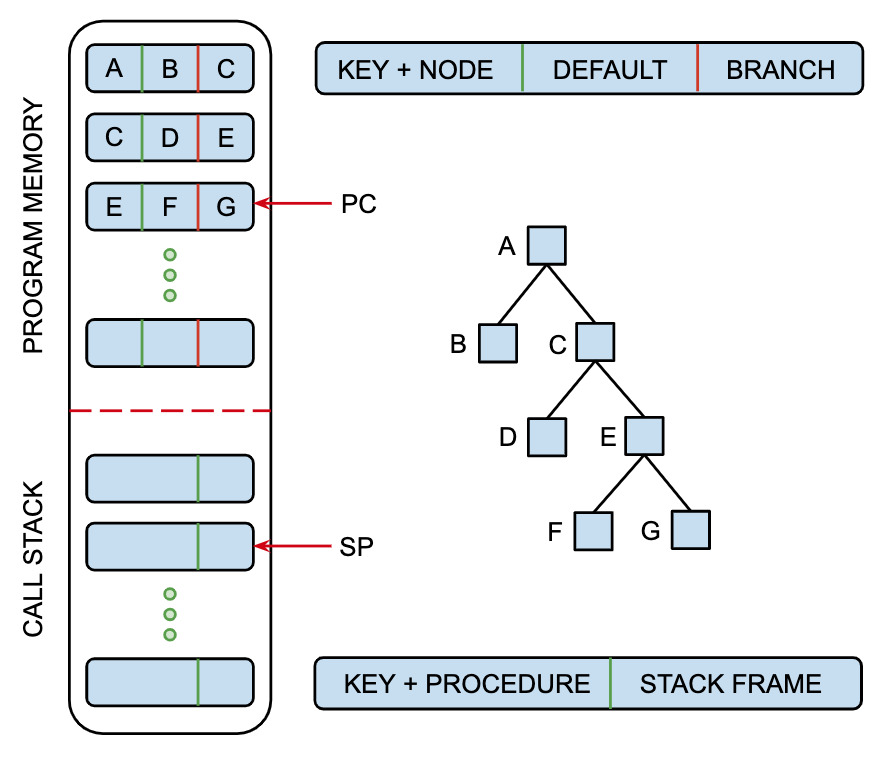
\includegraphics[width=5.9375in]{./figures/Differentiable_Structured_Programs.png} % 625 × 528 pixels
    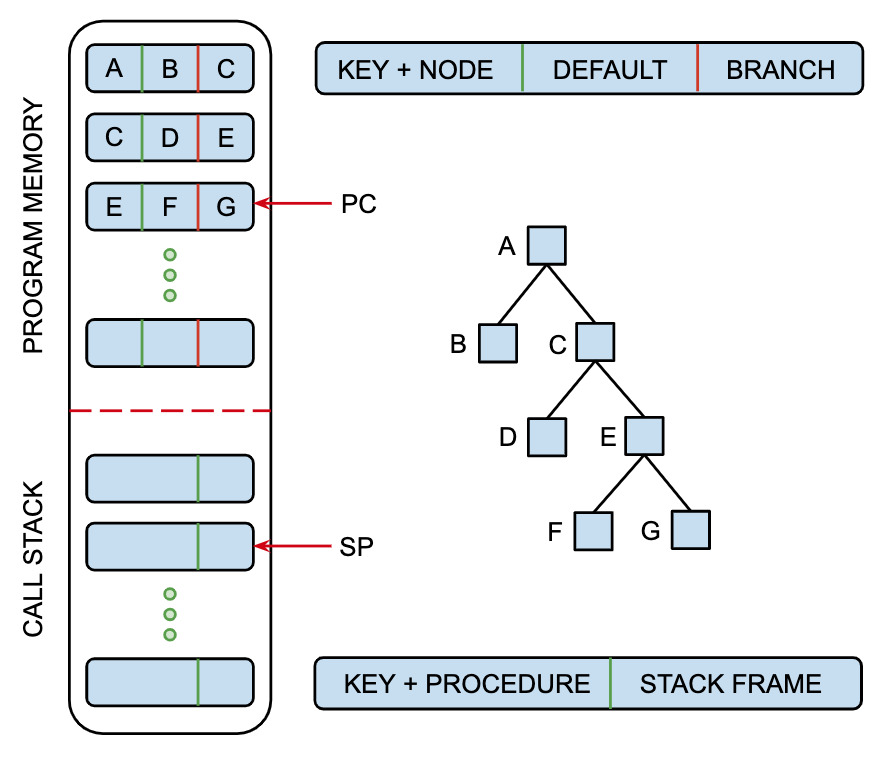
\includegraphics[width=3in]{./figures/Differentiable_Structured_Programs.png} % 625 × 528 pixels
  \end{center}
%
  \caption{We use pointers to represent programs as abstract syntax trees and partition the NTM memory, as in a conventional computer, into program memory and a LIFO execution (call) stack to support recursion and reentrant procedure invocations, including call frames for return addresses, local variable values and related parameters. The NTM controller manages the program counter and LIFO call stack to simulate the execution of programs stored in program memory. Program statements are represented as embedding vectors and the system learns to evaluate these representations in order to generate intermediate results that are also embeddings. It is a simple matter to execute the corresponding code in the FIDE and incorporate any of the results as features in embeddings.}
%
  \label{fig_programs}
%
\end{figure}

%%% %%%%%%%%%%%%%%%%%%%%%%%%%%%%%%%%%%%%%%%%%%%%%%%%%%%%%%%%%%%%%%%%%%%%%%%%%%%%

To support this hypothesis, we are developing distributed representations for programs that enable the apprentice to efficiently search for solutions to programming problems by allowing the apprentice to easily move back and forth between the two paradigms, exploiting both conventional approaches to program synthesis and recent work on machine learning and inference in artificial neural networks. Neural Turing Machines coupled with reinforcement learning are capable of learning simple programs~\cite{GravesetalCoRR-14}. We are interested in representing structured programs expressed in modern programming languages. Our approach is to alter the NTM controller and impose additional structure on the NTM memory designed to support procedural abstraction. 

%%%%%%%%%%%%%%%%%%%%%%%%%%%%%% END PROCEDURAL MODEL %%%%%%%%%%%%%%%%%%%%%%%%%%%%
